\chapter{Implementation and Processing Pipeline}\label{cap:implnprocpipe}
Chapter 4 describes how the proposed architecture was implemented in the working prototype. The discussion follows the data path from headset acquisition to teacher-facing visualization, with emphasis on the practical processing steps that make live engagement feedback possible during a lesson.



\section{Signal Acquisition Process}\label{sect:signacqproc}
Signal acquisition takes place on the Raspberry Pi paired with each headset. In practice, the acquisition runtime acts as a bridge between the Unicorn device and the LSL network. It prepares the required native libraries, opens the EEG device, receives samples through the vendor API, and publishes the resulting stream so that it can be discovered by the teacher workstation. Using LSL for this boundary follows its role in synchronized multimodal recording and local network stream discovery \cite{Kothe2025}.


At startup, the runtime verifies the environment required for LSL streaming and initializes the Unicorn acquisition path. The native library is loaded through Python bindings to the C API, with the required function signatures defined before the device is accessed. Available devices are then discovered, and the selected headset is opened. When no serial number is provided, the first available device is used, which is convenient for simple testing while still allowing explicit selection in a larger setup.


After the device is opened, an LSL outlet is created and descriptive metadata is attached to it. This metadata includes information such as the student label, device name, stream identity, and channel description. Although these fields are not part of the EEG signal itself, they are necessary for a multi-user classroom interface, where several streams must be displayed in a readable and unambiguous way.


During acquisition, samples are read repeatedly from the headset and pushed to the LSL outlet. Engagement is not computed on the Raspberry Pi. Keeping the acquisition loop limited to reading and publishing makes the student-side process shorter and more predictable, while preserving the raw values for the teacher application. If acquisition is interrupted, the runtime attempts to stop the device and release its handle, reducing the risk of leaving the hardware in an inconsistent state for the next session.


Deployment support is part of this pipeline as well. The teacher application can copy the runtime and required vendor files to the Raspberry Pi and prepare the Python environment used by the acquisition node. This is important for a system intended to work with several nodes, because each one must be configured in a consistent way before being used in a lesson.


On the workstation, a background collector completes the acquisition path. It discovers LSL streams, opens receiving inlets, reads available sample chunks, and stores each stream in a structured state. Identification metadata, connection freshness, packet count, latest raw value, latest engagement value, and short-term histories are kept together so that the dashboard can use live data without managing network streams directly.


Responsiveness is especially important because Streamlit reruns page logic frequently. Long-running acquisition work cannot depend on a single page render. By collecting data in the background and exposing snapshots to the interface, the implementation separates continuous signal reception from visual refresh. This makes the live display more reliable and keeps the interface logic easier to follow.

\section{Data Filtering Procedures}\label{sect:datafiltproc}
Filtering is intentionally kept modest in the current prototype. The system does not implement a full laboratory EEG preprocessing chain. Instead, it performs the steps needed for the engagement metric: selecting the relevant channel, buffering samples into analysis windows, removing the constant offset, and estimating spectral content. This reflects the practical compromise often required when portable EEG is used outside controlled laboratory environments \cite{Xu2018}.


Processing begins with basic validation of the incoming sample. Empty values or values that cannot be converted to a numeric form are ignored, which protects the rest of the pipeline from malformed input. This choice keeps the collector robust without adding complex error handling to the real-time path.


Selected values are buffered until enough recent data is available for frequency analysis. Once a processing window is formed, its mean is subtracted. Removing this constant component prevents the engagement estimate from being influenced by a simple voltage offset rather than by variation in the signal.


Frequency-domain analysis is then performed using an FFT. Rather than reconstructing separate filtered signals for each band, the implementation estimates the power contained in the theta, alpha, and beta ranges directly from the transformed window. This approach is compact and suitable for the prototype, because the final metric depends on relative spectral power rather than on the detailed time-domain shape of each band.


Figure~\ref{fig:eeg_processing_pipeline} summarizes the processing path. Incoming samples are first checked and buffered. Once a complete window is available, the mean is removed, spectral power is estimated in the relevant EEG bands, and the beta-to-alpha-theta ratio is converted into the displayed engagement value through scaling, smoothing, and calibration.

\begin{figure}[h]
\centering
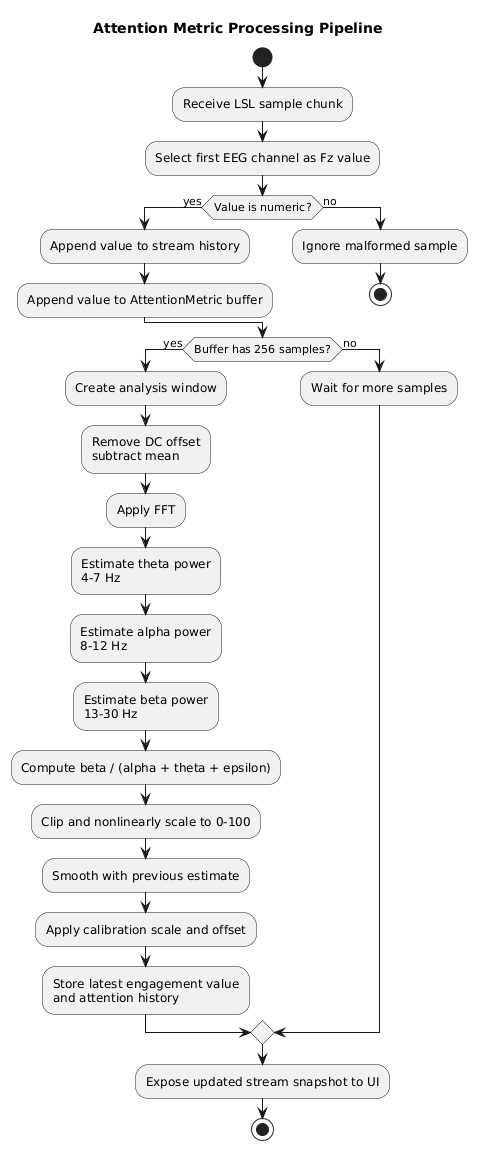
\includegraphics[width=0.82\textwidth,height=0.68\textheight,keepaspectratio]{En/UML_eeg_pipeline.png}
\caption{Processing pipeline used to transform incoming LSL samples into the displayed engagement value.}
\label{fig:eeg_processing_pipeline}
\end{figure}
Not all EEG artifacts are removed by this procedure. Eye movements, muscle activity, poor electrode contact, and normal classroom movement may still influence the signal. This limitation is accepted because the system is a feasibility prototype for real-time classroom feedback, not a clinical acquisition platform. To keep the process transparent, raw sample history is still preserved in the interface, allowing the underlying signal to be inspected when needed.


A short processing path also makes the implementation easier to explain. The relationship between the incoming samples and the displayed engagement value remains understandable, which is important in a dissertation prototype. A more complex black-box pipeline might improve some aspects of signal handling, but it would also be harder to validate and justify within the scope of this work.

\section{Attention Metric Extraction}\label{sect:attmetrextr}
Attention metric extraction converts each prepared EEG window into a bounded engagement value. The metric is implemented as a separate processing component, independent of the Streamlit pages, so that the mathematical logic remains clear and can be adjusted without rewriting the interface.


For each window, spectral power is estimated in the theta, alpha, and beta bands. These bands are commonly used in EEG interpretation and have also been used in attention-related feature comparisons \cite{Niedermeyer2005,Liang2022}. The metric compares beta activity with lower-frequency activity using a beta-to-alpha-theta ratio, following the engagement index evaluated by Pope et al. \cite{Pope1995}:
\[
ratio = \frac{P_{\beta}}{P_{\alpha} + P_{\theta} + 10^{-6}}
\]
where \(P_{\beta}\), \(P_{\alpha}\), and \(P_{\theta}\) represent the estimated band powers. The small constant prevents division by zero.


This ratio is converted into a percentage-like score through clipping and nonlinear scaling. Smoothing is then applied using the previous estimate, which prevents the displayed value from changing too abruptly during a lesson. Finally, calibration parameters are applied and the result is clipped to the display range used by the interface.


In this work, the metric is understood as a practical engagement indicator, not as a precise measurement of attention. EEG-based attention estimates are sensitive to noise, artifacts, and individual differences. For that reason, the value is used to support classroom reflection rather than to produce definitive conclusions about a student. This interpretation follows the wider caution in portable EEG and wearable engagement research \cite{Xu2018,BustosLopez2022}.


Once computed, the engagement value is stored together with the corresponding stream state. The same value can then be reused by compact cards, detailed inspection views, and report summaries. This avoids unnecessary recalculation during interface refreshes and keeps all views consistent with the same underlying stream state.

\section{Visualization Interface}\label{sect:visint}
For the teacher-facing interface, the implementation uses a Streamlit application organized around the main workflow of the system. From the dashboard, the teacher can access lesson creation, teaching, reports, and administration. This arrangement keeps the entry point approachable and avoids exposing low-level acquisition details before they are needed.


Lesson creation handles the preparation of teaching materials. Uploaded files are stored locally, registered in a material manifest, and checked for duplicates using a file hash. PDF files can be used directly, while supported presentation formats can be converted into PDF previews when LibreOffice is available. For compatible PowerPoint files, speaker notes are extracted and stored so that they can be shown later in presenter view.


The Create Lesson screen in Figure~\ref{fig:create_lesson} represents this preparation stage. The upper part of the page handles the upload and title input, while the saved-materials table confirms what has already been registered locally and whether a preview is available.

\begin{figure}[h]
\centering

\includegraphics[width=0.9\textwidth]{\detokenize{En/4. Create Lesson.png}}
\caption{Create Lesson page used to upload teaching material and inspect saved materials.}
\label{fig:create_lesson}
\end{figure}
During teaching, saved materials are presented through a browser-based slide interface. The page supports presenter view with notes, presentation-only mode, keyboard navigation, page counters, and a separate audience window. As a result, the teacher can run the lesson from the same application that receives engagement information.


Figure~\ref{fig:teach_lesson} shows the teaching stage of the workflow. The teacher selects a saved material, chooses the presentation mode, and starts the lesson from the same interface used for engagement monitoring. This keeps lesson delivery and signal observation within one application context.

\begin{figure}[h]
\centering

\includegraphics[width=0.9\textwidth]{\detokenize{En/5. Teach Lesson.png}}
\caption{Teach Lesson view showing material selection, presentation controls, and presenter-oriented lesson delivery options.}
\label{fig:teach_lesson}
\end{figure}
Combining presentation and monitoring is important for usability. A classroom workflow becomes harder to manage if slides, EEG streams, and post-lesson review are spread across unrelated tools. By placing these actions in one application, the prototype reduces context switching and makes neurofeedback function more like a teaching aid than an experiment control panel.


Live stream visualization uses compact student cards together with a detailed inspection view. Cards show the current engagement value, device label, stream label, packet freshness, and status. The detailed view adds raw signal charts, packet counts, stream metadata, and a larger engagement display. This two-level structure keeps the classroom view simple while still providing enough information for validation and troubleshooting.


After a lesson, the reports page provides a structured view of engagement by lesson part. Results are shown both as a chart and as a table, allowing the teacher to observe general trends and inspect exact values. In this way, live monitoring is transformed into material that can be reviewed after the teaching session.


The report view in Figure~\ref{fig:reports_page} is designed for quick post-lesson interpretation. The chart gives an immediate comparison between lesson parts, while the table keeps the numerical values visible for documentation or later analysis.

\begin{figure}[h]
\centering

\includegraphics[width=0.9\textwidth]{\detokenize{En/6. Reports.png}}
\caption{Reports page summarizing engagement by lesson part as both a chart and a table.}
\label{fig:reports_page}
\end{figure}
Reporting is intentionally concise. Its purpose is not to overwhelm the teacher with raw physiological data, but to present a summary that can support lesson revision. A chart can quickly show whether a lesson part was associated with lower engagement, while the table keeps the corresponding numerical values available for closer inspection.


Setup and maintenance tasks are placed in the administration page so they do not interfere with normal teaching. This page includes Raspberry Pi inventory, network scanning, deployment support, stream validation, deployment logs, and PIN management. Separating these tools from the teaching interface keeps technical preparation available without making it part of the everyday classroom view.

\section{Scalability}\label{sect:scal}
The prototype was designed as a distributed system where each student station works independently using one EEG headset and one Raspberry Pi node. Communication between nodes is handled through Lab Streaming Layer, which allows EEG streams to be discovered automatically by the teacher workstation.

This design makes the system easier to extend in a classroom environment. New students can be added by connecting additional acquisition nodes without requiring major changes to the existing setup. Because acquisition, processing, and visualization are separated into different components, issues affecting one node do not stop the entire system.

The processing pipeline was also designed to support multiple users at the same time. Engagement estimation is calculated independently for each stream using buffered analysis windows, allowing the workload to increase gradually as more users are connected. Since the calculations mainly involve lightweight signal processing operations, the hardware requirements remain relatively low.

The Streamlit dashboard follows the same modular structure by maintaining separate states for each connected stream. This organization makes future extensions easier, including support for additional engagement metrics, classroom grouping, or lesson analysis features.

At the current stage of development, the architecture appears flexible enough to support further testing and expansion in classroom scenarios.

\clearpage
